\chapter{引言}


\section{研究背景}

随着互联网技术的不断发展,社交网络已经成为人们日常生活中不可或缺的一部分。人们可以通过社交网络获取新闻,与他人进行交流互动,发布个人信息等等。对于大多数中国互联网用户来说,QQ、微博、微信、陌陌等社交应用是其日常上网的主要应用。根据中国互联网络信息中心(CNNIC)的调查结果显示\cite{internetSurvey},有79.5\%的用户每天上网的时间达到两个小时以上,而其中77.0\%的时间是用在社交应用上。社交网络使得人们不再受报刊、电视等信息来源的限制,拥有了更多获取信息的渠道。

\begin{figure}[h] 
  \centering
  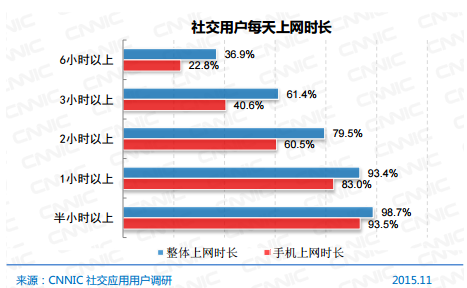
\includegraphics[height=8cm]{InternetUsingTime}
  \caption{社交用户每日上网时长\cite{internetSurvey}}
  \label{InternetUsingTime}
\end{figure}

对于信息发布者来说,社交网络给他们提供了一个新的推广和营销平台。由于大量用户花费大量时间在社交网络中,传统的信息发布渠道日渐衰落,而社交网络凭借其传播范围广、扩散速度快、受众数量大、推广形式多等特点,逐渐成为一种全新的、重要的、高效的推广方式。Shama Hyder在《网络社交媒体营销》一书中提到社交媒体必将取代传统媒介成为营销推广的主要手段 \cite{hyder2016zen}。

利用社交网络进行推广营销,能够在短时间内将信息传递给目标群体。在微博、微信公众号等社交平台上,流行用户往往拥有几百万甚至几千万的关注量,其发布的每一条消息都有大量的用户关注。且传播速度快,实时发送接收,还能够根据受众的不同发布不同的信息,使得推广行为更加具有针对性。同时,利用社交网络进行推广,形式上更加灵活多样,利用文字、图片、语言、视频的手段,能够更加充分地进行展示。优秀的推广内容甚至能够通过用户自发进行传播,呈现爆发式营销增长。社交网络公司Facebook,在2016年广告业务的总收入达到268亿美元\cite{Facebook}。而微博在2016年Q4季度中,其广告收入也达到了1.879亿美元\cite{微博}。这仅仅是这两家社交网络公司自身的广告营销收入,其最大的贡献是为其用户提供了一个社交网络的营销平台,由此产生的推广营销效益更加巨大。

由于社交网络推广方式的灵活性,对于商品、活动、人物等众多对象均可以进行推广,本文主要研究的是演员针对影视剧在社交网络上的推广。影视剧的关注人群广泛,且娱乐性、话题性强,能够更好地适用社交网络上的多种推广模式。

随着大数据、机器学习等技术的不断进步,社交网络在影视剧推广方面的重要作用越来越不容忽视。以国产电影《失恋33天》的社交网络营销为例,该部电影在2011年上映,凭借成功的网络营销手段,取得3.5亿人民币的优秀票房,是原预估票房的十倍以上\cite{熊莉2012失恋}。这部电影以新浪微博、腾讯微博等社交网站为重要推广平台,打造了拥有近10万粉丝量的官方微博,并创建了众多热门话题,通过宣传短片、制造话题等众多手段,针对网络用户的特点精准投放营销策略,并引导用户参与话题讨论,通过转发、评论等手段,将用户自身的社交网络融入到宣传网络当中,进一步扩大了宣传效果。在日后的各类总结点评中,《失恋33天》都被认为是电影营销手段的一次最成功的创新,利用社交网络对影视剧进行推广的方法从此日益发展。

通过对现有社交网络推广案例进行分析即可发现,目前针对影视剧的网络营销手段层出不穷,而且还存在着继续增多的趋势。例如宣传方会在微博、QQ、微信等社交媒体上创建官方账号,发布关于影片的文字、图片消息,演员消息,宣传短片等。这样的宣传方式会在影片上映前后持续较长时间,吸引大量粉丝关注,提高影片关注度。例如电影《嫌疑人X的献身》,其在微博上的官方账号共发布了744条微博,拥有62万粉丝关注,发布的每条微博有数千条的转发、评论、点赞\footnote{http://weibo.com/p/1002065746403567}。

\begin{figure}[h] 
  \centering
  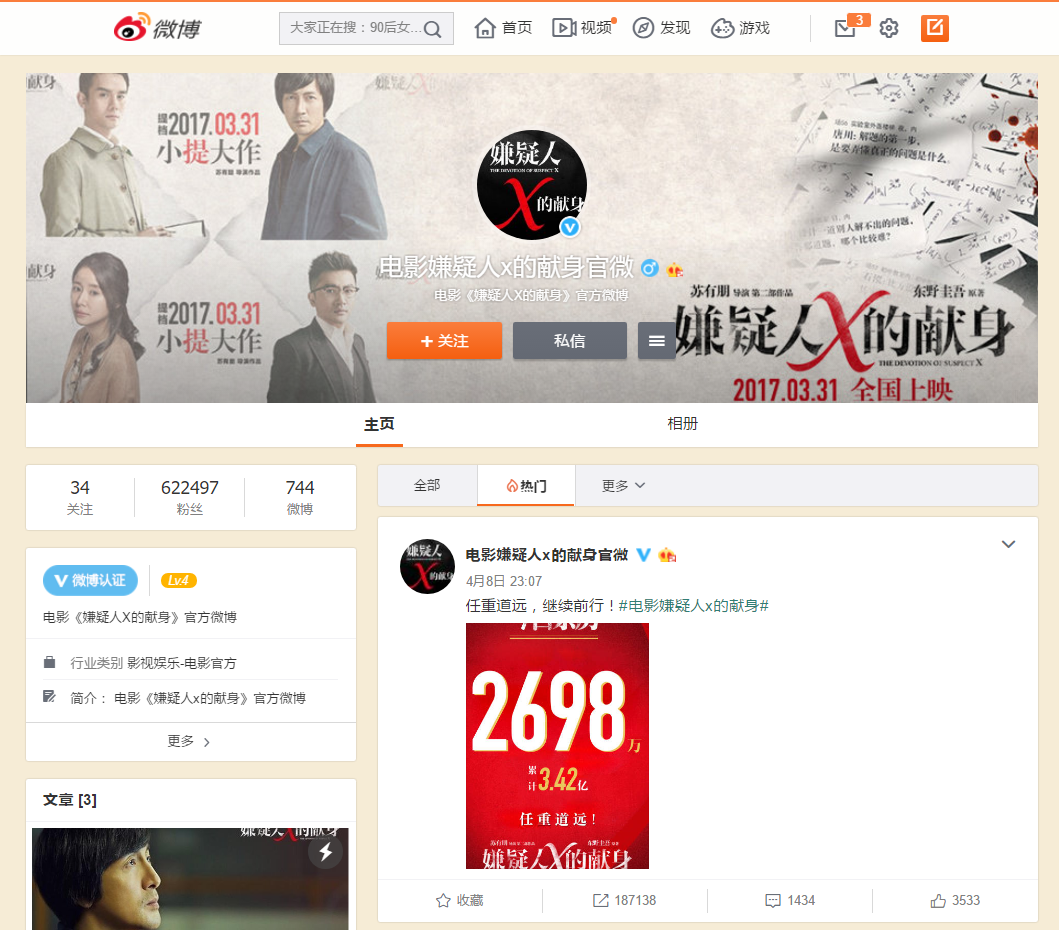
\includegraphics[height=10cm]{嫌疑人}
  \caption{《嫌疑人X的献身》官微截图}
\end{figure}

同时,宣传方还会在社交网络上制造影视剧相关话题,并不断推高话题热度,扩大影片影响力。例如电影《致青春》在网络营销中通过推出“回忆青春”活动、推出主题曲、制造“有一种感情叫赵薇黄晓明”等流行语的形式制造多个热点话题,激发用户自动传播,最终实现病毒式传播效果。另外宣传方还可以通过各类影评、新闻报道提升观众的观看热情。例如,电视剧《人民的名义》在豆瓣网可以找到近4万篇影评\footnote{https://movie.douban.com/subject/26727273/},短短一周之内在微信公众号上即出现了55篇与其有关的阅读量超过10万的文章,这样的推广方式能够为影视剧打造良好的口碑,塑造良好形象,吸引更多观众观看。

而网络推广的各种营销手段,往往是通过一些关键节点传播和扩散给广大用户,这些节点一般是由影视剧的官方账号、演员或者经过社交平台验证的“大V”用户组成。这些用户拥有巨大的粉丝量,能够将各类宣传消息推送给众多的用户,起到宣传媒体的作用\cite{kwak2010twitter}。

影视剧演员往往拥有众多粉丝,关于演员的新闻报道和演员自身发布的消息都能够获得极高的关注度,演员在社交网络中具有较高的影响力\cite{shafiq2013identifying},是影视剧宣传推广的重要节点。影视剧演员可以通过自身的影响力在社交网络上制造话题,通过发布各种类型的消息,包括文字、图片、音视频等等,或者利用其它用户发布关于自己的新闻报道,引起关注自己的粉丝的广泛反响,引发热烈讨论。然后根据网络话题演化的规律\cite{he2009detecting},在适当时刻不断推高话题热度,使其成为热点,获得更多受众。

但是在进行推广时,不同的推广方式会收到不同的推广效果,不同的用户使用同样的推广方式也会得到不同的结果。如图~\ref{蒋欣}所示,演员蒋欣在对其主演的电视剧《欢乐颂》进行宣传时,发布了两条微博,但是其转发和点赞数量却有很大的不同。可想而知,这两条微博能够获得的推广效果也是截然不同的。

\begin{figure}[h]
  \centering%
  \subcaptionbox{转发:7186 评论:25817 点赞:143036}
    {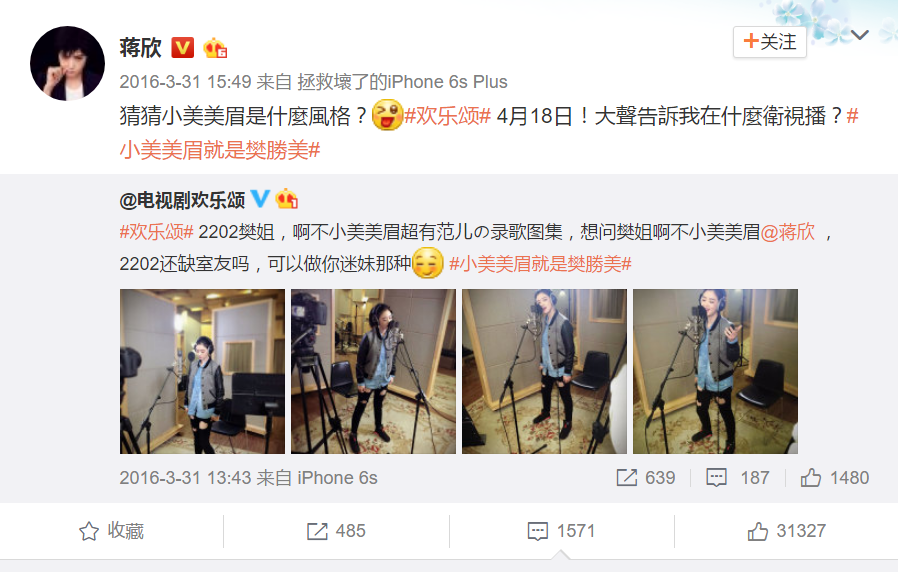
\includegraphics[height=4.5cm]{蒋欣1}}
  \subcaptionbox{转发:485 评论:1571 点赞:31327}
      {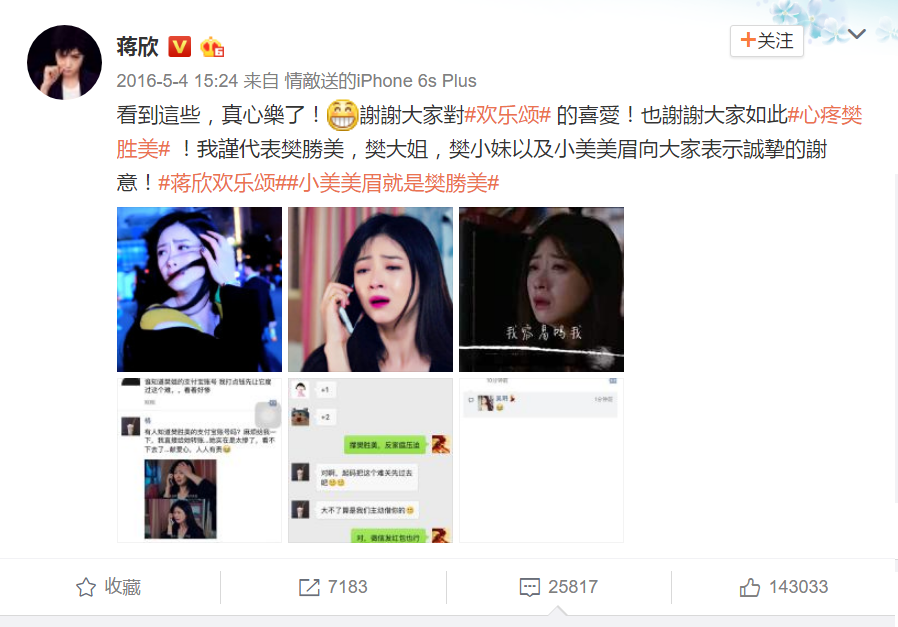
\includegraphics[height=4.5cm]{蒋欣2}}
  \caption{不同微博的推广效果比较}
  \label{蒋欣}
\end{figure}

另外,对电影和电视剧的推广有很大差异。例如,对于电影的推广来说,由于其属于一次性消费,只需要吸引观众进入影院观看即可。而对于电视剧的推广来说,由于其播放周期较长,需要对用户维持长时间的粘滞力,在吸引新用户进行观看的同时,还要保持老用户的持续关注。因此,对于电影和电视剧的推广手段就需要有不同的侧重点,需要有针对性地采用不同的推广方式。目前关于电影推广的研究较为常见,由于电影的高投入高产出性,宣传方也会投入更多精力关注电影推广。而关于电视剧有针对性的推广研究较少,推广方式也较为有限,需要给予更多的关注。

因此,为了能够获得更好的推广效果,最大限度地发挥社交网络的推广作用,本文选取演员在社交网络上的对于电视剧的推广微博作为研究对象,根据演员自身和待推广电视剧的特点,分析不同推广策略带来的不同的微博影响力,识别出最有效的推广策略。

\section{主要研究内容和挑战}

本文的数据来源是爱奇艺、豆瓣和微博,获得电视剧相关、演员相关的所有基本信息和社交行为信息,如电视剧官方微博数据、电视剧话题数据、演员粉丝量、演员发布的所有微博信息等等,并对这些数据进行了整理和分析。

首先针对这些数据进行了一些测量,比如基于粉丝参与度(微博转发量、评论量、点赞量)提出微博影响力指数,来衡量一条微博能达到的推广效果,进而能获得演员发布关于电视剧的微博的总体微博影响力;测量电视剧微博话题热度与微博影响力之间的相关性,静态数据和动态数据都说明了二者的高度相关性,从而利用微博影响力来刻画话题热度,等等。

进而,从数据中识别出演员推广电视剧的相关模式,包括演员在电视剧不同时期的推广特点,不同时间的推广特点,发布形式上的互动特点等,其中还包括一些演员推广过程中的时空行为模式,如虽然有很多演员在微博上并不活跃,但是几乎所有演员都会在电视剧上映前后几天发布推广微博;发现大部分演员都在很短的时间内对官微“@”自己的微博进行响应等等。

最后利用倾向值匹配模型对演员在社交平台上的推广行为进行分析建模。对各个推广策略与推广效果之间的因果关系一一进行分析,识别电视剧推广的最有效的策略。并且在这个过程中不断进行优化,在应用模型时引入了更多的混淆变量,更充分地考虑各种推广效果的影响因素,同时结合电视剧话题在微博上的演化规律,对演员的推广行为进行分段处理,更精准更合理地识别有效策略。另外,还对模型进行了显著性检验和平衡性检验,验证了该模型的适用性和准确性。

本文所述研究主要存在如下几方面挑战:

\begin{itemize}

\item[(1)]目前基于社交媒体数据的研究主要集中在电影领域,关于电视剧的研究较少,且关于电影的研究主要是结合社交数据进行票房预测,很少集中在推广领域。同时,电影是一次性消费,而电视剧是一个持续性消费,除了首播前的宣传,当电视剧开播后,在维持现有观众群、防止用户流失的同时还要吸引更多人来观看。由于电视剧播出周期长、用户行为复杂等问题,电视剧相关的研究往往被忽略。关于电视剧在社交网络上的推广行为的研究更是少有相关工作可以参考,但是微博作为电视剧推广的重要平台,好好利用能达到事半功倍的效果。

\item[(2)]理想情况下,检验策略有效性的黄金标准是基于实验的方法,比如做A/B测试,但是随机对照实验成本高,随机选取用户随机分配策略可操作性非常低,实际情况下中不可实现。因此提供一个基于观测数据的统计方法而不是实验方法来检测策略的有效性是非常重要和有必要的。

\item[(3)]采用非随机对照实验的方法结果会受到混淆变量的影响,容易出现数据偏倚、组间基线不齐等问题。如何排除混淆变量的影响,得到推广策略和推广效果之间的净效应也是一个难点。例如如果直接选用回归关系,一是推广策略与推广结果不一定是线性关系,二是混淆变量可能与推广策略和推广结果都有关系,可能有共线性问题。

\item[(4)]数据获取难度大。在微博上有大量用户,从中识别并获取全部与电视剧相关的微博比较困难。同时如何仅根据电视剧基本信息,获取与其对应的电视剧官方账号和演员在微博中id,以及获得id后如何在非好友、无权限的情况下爬取他们的全量数据,都是有待解决的问题。


\end{itemize}

\section{主要贡献和组织结构}

针对以上的问题与挑战,本文选取演员发布的微博作为研究对象,更有代表性和针对性,利用倾向值匹配模型,将混淆变量纳入Logistic模型,归纳成一个倾向值,进行倾向值匹配时,用以控制混淆变量,使得对最终结果的影响只能归因于自变量,从而评估出演员推广电视剧的有效策略。本文的主要贡献如下:

\begin{itemize}

\item[(1)]本文不但做了一些分析和测量工作,提出相关评价指数,可以指导未来研究,如基于粉丝参与度提出微博影响力指数,提出电视剧微博话题热度指数等等;还总结归纳出演员对电视剧的推广模式和推广策略及其特点,并发现了一些演员推广过程中的时空行为模式,如一种常见推广模式是电视剧官方微博作为话题的源头来发布微博,同时"@"其他演员,然后其他演员通过转发微博来响应官微,来扩大微博影响力。

\item[(2)]本文利用倾向值匹配模型对演员在社交平台上的推广行为进行建模和因果分析。不但解决了随机对照实验成本高、操作性低等问题,还解决了可能出现的选择偏倚、混淆变量影响等问题。对各个推广策略与推广效果之间的因果关系一一进行分析,排除混淆变量的影响,分析推广策略与推广效果之间的净效应,识别电视剧推广的有效策略。还对模型进行了显著性检验和平衡性检验,验证了该模型的适用性和准确性。而且在以往的研究中,倾向值匹配算法多用于医药学、社会学和经济学等领域,在社交媒体大数据领域的应用较少,本文的应用开拓了一种新的应用方向。

\item[(3)]本文根据电视剧话题在微博上的话题演化规律,提出基于话题时序演化的改进模型。对演员的推广行为进行分段研究,更精准更合理地识别有效策略。因为在电视剧的不同时期,演员的推广特点和推广侧重点有所不同。在电视剧拍摄期间,演员会发布电视剧拍摄相关的信息如拍摄进度、角色定妆照等,电视剧首映前,演员会发布微博提醒粉丝们电视剧的首映时间,电视剧上映时,他们会发布更多的微博讨论电视剧角色、剧情等。因此,对演员的推广行为进行分段研究更具有指导意义。

\item[(4)]为了避免获取全部微博数据产生的海量数据,本文选取演员发布的推广微博作为研究对象。不但使研究更有代表性和针对性,还有效降低了实验数据量。在数据获取过程中,采用多种方法和技术获取数据,包括模拟搜索、模拟登陆、抓取手机端数据而非电脑端数据等方法,解决了非好友、无权限下无法获取数据和获取速度慢的问题。

\end{itemize}

本文的组织结构如下:

第二章主要介绍研究现状和相关工作,包括当前关于影视剧和社交网络相结合的研究情况,因果分析的主要研究方法,以及基于倾向值匹配的因果分析方法的发展和应用情况。

第三章主要介绍本文所使用的实验数据集,包括数据的来源、收集方法和数据形式。同时还介绍了基于该数据集进行的一些基础分析、测量和从中挖掘出的数据特征和规律等。

第四章主要介绍了倾向值匹配算法的原理、具体算法步骤以及对模型的验证方法。

第五章将倾向值匹配算法应用到数据集上,对不同的推广策略进行了比较分析,并提出了一种改进模型,验证了该算法对推广策略分析的适用性和准确性。

第六章是对全文的总结,以及对下一步工作的展望。




































